%  Template for ICASSP-2021 paper; to be used with:
%          spconf.sty  - ICASSP/ICIP LaTeX style file, and
%          IEEEbib.bst - IEEE bibliography style file.
% --------------------------------------------------------------------------
\documentclass{article}
\usepackage{spconf,amsmath,graphicx,hyperref}

% Example definitions.
% --------------------
\def\x{{\mathbf x}}
\def\L{{\cal L}}

% Title.
% ------
\title{AIML 425 Assignemnt 1}
%
% Single address.
% ---------------
\name{Quan Zhao (Student ID: 300471028)}
%\name{Author(s) Name(s)\thanks{Thanks to XYZ agency for funding.}}
\address{Victoria University of Wellington}
%
% For example:
% ------------
%\address{School\\
%	Department\\
%	Address}
%
% Two addresses (uncomment and modify for two-address case).
% ----------------------------------------------------------
%\twoauthors
%  {A. Author-one, B. Author-two\sthanks{Thanks to XYZ agency for funding.}}
%	{School A-B\\
%	Department A-B\\
%	Address A-B}
%  {C. Author-three, D. Author-four\sthanks{The fourth author performed the work
%	while at ...}}
%	{School C-D\\
%	Department C-D\\
%	Address C-D}
%
\begin{document}
%\ninept
%
\maketitle
%
\section{Introduction}
\label{sec:intro}

Generative models are a subset of machine learning models designed to capture and mimic the underlying distribution of the data on which they are trained. They can produce new samples that resemble the input data but might not have been part of the original training set.

In this work, I will present my understanding of training and tuning generative models.

Three models will be trained:

1. $f1$, $(2D)Z\sim N(0,1) \rightarrow (2D)Y\sim U(0,1)$

2. $f2$, $(2D)Y\sim U(0,1) \rightarrow (2D)Z\sim N(0,1)$

3. $f3$, $(1D) Y\sim U(0,1) \rightarrow (2D) Z\sim N(0,1)$

We have introduced experiments to discuss:

  - The effects of varying levels of L2 regularization on the weights for $f1$.
  
  - The implications of concatenating the two networks, $f1$ and $f2$.

  - Display the point mapping from model $f3$'s input to its output.

% Below is an example of how to insert images. Delete the ``\vspace'' line,
% uncomment the preceding line ``\centerline...'' and replace ``imageX.ps''
% with a suitable PostScript file name.
% -------------------------------------------------------------------------
% \begin{figure}[htb]
%   %
%   \begin{minipage}[a]{.48\linewidth}
%     \centering
%     \centerline{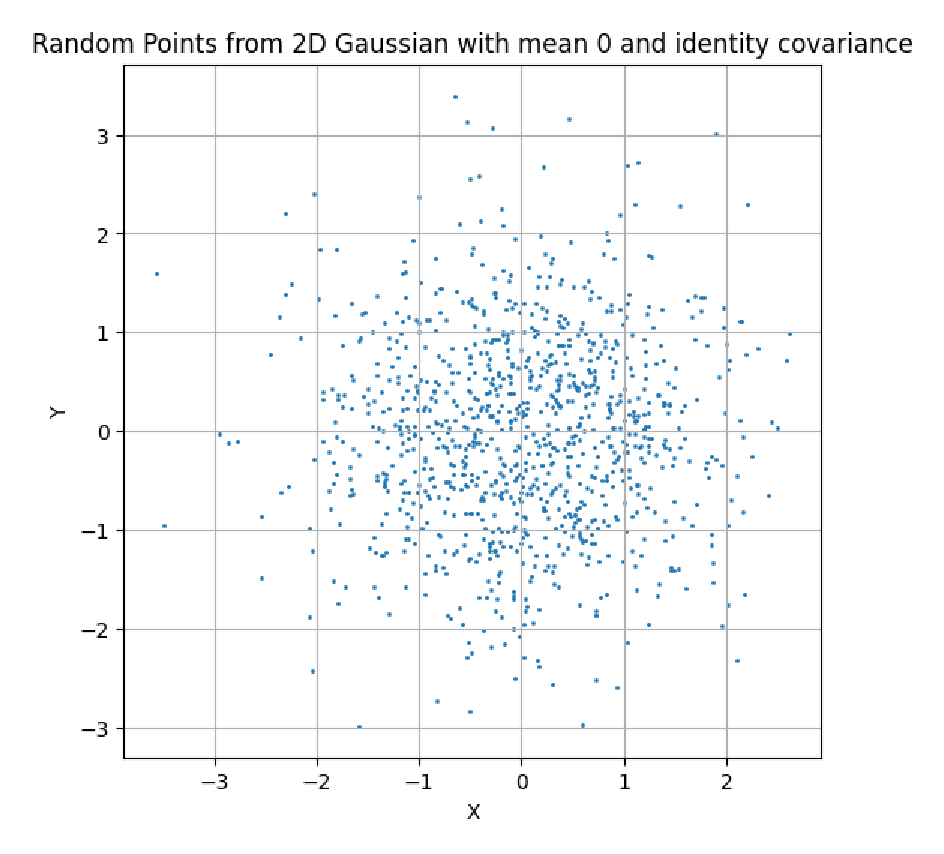
\includegraphics[width=3.0cm]{images/gaussian2d}}
%   %  \vspace{1.5cm}
%     \centerline{(a) 2D Gaussian distribution}\medskip
%   \end{minipage}
%   \hfill
%   \begin{minipage}[c]{0.48\linewidth}
%     \centering
%     \centerline{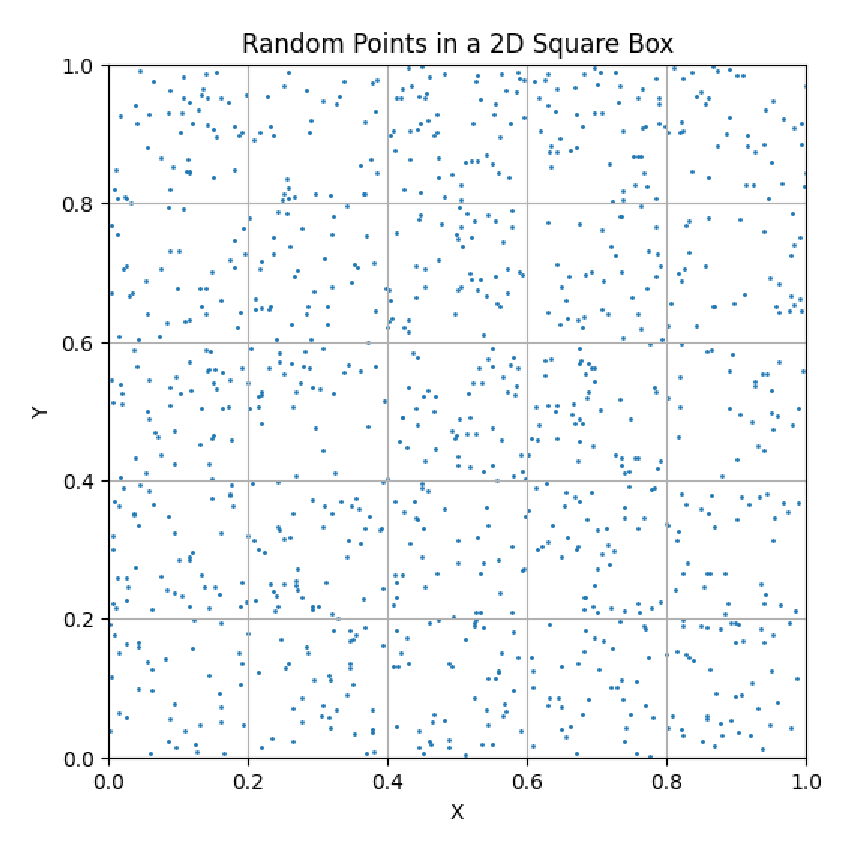
\includegraphics[width=2.7cm]{images/uniform2d}}
%   %  \vspace{1.5cm}
%     \centerline{(b) 2D uniform distribution}\medskip
%   \end{minipage}
%   %
%   \caption{Data distribution plots}
%   \label{fig:res}
%   %
%   \end{figure}
  

\section{THEORY}
\label{sec:theory}

\subsection{MMD}
\label{ssec:mmd}

Maximum Mean Discrepancy (MMD) \cite{gretton2012kernel} is a statistical test for determining whether two samples come from the same distribution. It's often used in the context of kernel methods and has applications in training generative models.

$ \text{MMD}^2 = E[k(x, x')] + E[k(y, y')] - 2E[k(x, y)] $

where, $k(.,.)$ is the kernel function. 
$x, x'$ are independent samples from $X$,
and $y, y'$ are independent samples from $Y$.

% \subsubsection{Kernel}
% \label{sssec:kernel}

A common choice of kernel for MMD is the Gaussian (RBF) kernel:

$ k(x, y) = \exp\left(-\frac{||x - y||^2}{r}\right) $
Where, $r$ is chosen by designer



\subsection{L2 Regularization}
\label{ssec:l2regularization}

L2 regularization \cite{rumelhart1986learning} introduces a penalty on the squared magnitudes of model weights. 
In Nerual Networks, the loss function with L2 regularization is:

$ J(\theta) = \text{MMD}(\theta) + \lambda ||\theta||_2^2 $

Where, $\lambda$ is the regularization strength
, $||\theta||_2^2$ is the L2 norm of the parameter vector.

\section{RESULTS}
\label{sec:results}

\subsection{Train a fully connected neural network f1 of your design that converts a
two-dimensional (2D) Z ~ N (0, I) into a 2D uniform Y . That is, Y has
a uniform density of 1 in a 2D square box (2-cube; edges have length 1).}
\label{ssec:q1}

A 3 fully-connected layers nerual network is been used train this model, 
which use MMD is Loss function with Gaussian Kernel. 
Gradient Descent Learning algorithms use Adam.
Regularization method is L2 regularization.

From Figure $\ref{fig:f1}$ we can see the input points are good mapping to the predicate points.

\begin{figure}[htb]

  \begin{minipage}[b]{1.0\linewidth}
    \centering
    \centerline{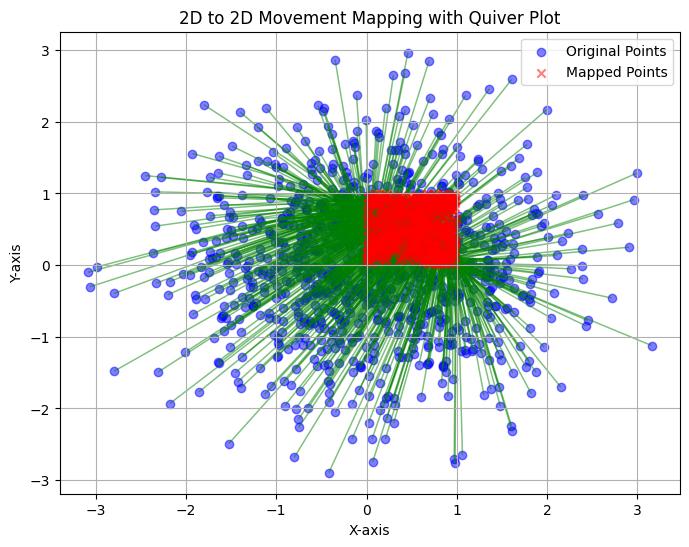
\includegraphics[width=4.0cm]{images/f1}}
  %  \vspace{2.0cm}
    \centerline{(a) Result 1}\medskip
  \end{minipage}
  %
  \caption{Points movement from input to predicate points}
  \label{fig:f1}
  %
  \end{figure}

\subsection{Train a second network f2 that converts the 2D Y into a Gaussian 2D Z}
\label{ssec:q2}

A 3 fully-connected layers nerual network is been used train this model, 
which use MMD is Loss function with Gaussian Kernel. 
Gradient Descent Learning algorithms use Adam.
Regularization method is Dropout.

\subsection{Train f1 with different levels of L2 regularization on the weights and discuss the effect.}
\label{ssec:q3}

We experimented with the $f1$ model using varying $L2$ values: $
1\times 10^{-1}$ to $1\times 10^{-20}$. 
Figure $\ref{fig:q3}$a depicts average loss across these values: 
sharp reduction post $1\times 10^{-2}$, 
stability after $1\times 10^{-4}$. 
Figures $\ref{fig:q3}$b-e show point mappings: 
initially to a point, then evolving to a line with 
increasing weight. Post $1\times 10^{-4}$, 
input-output mapping remains stable.

\begin{figure}[htb]

  \begin{minipage}[b]{1.0\linewidth}
    \centering
    \centerline{\includegraphics[width=5.0cm]{images/q3_1}}
   %\vspace{2.0cm}
   \centerline{(a) $f1$ Avg Loss with diff L2 weight decay }\medskip
  \end{minipage}
  %
  \begin{minipage}[b]{.48\linewidth}
    \centering
    \centerline{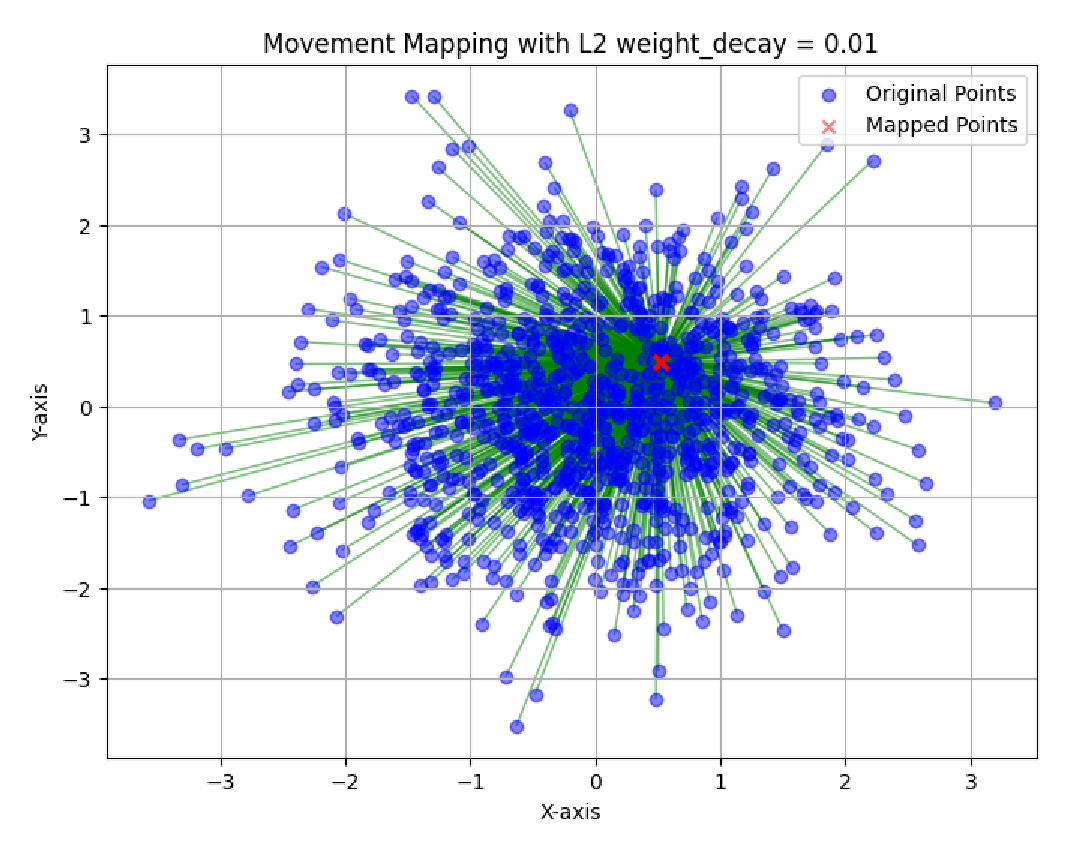
\includegraphics[width=2.5cm]{images/q3_1e-2}}
  %  \vspace{1.5cm}
    \centerline{(b) Points movement with 1e-2}\medskip
  \end{minipage}
  \hfill
  \begin{minipage}[b]{0.48\linewidth}
    \centering
    \centerline{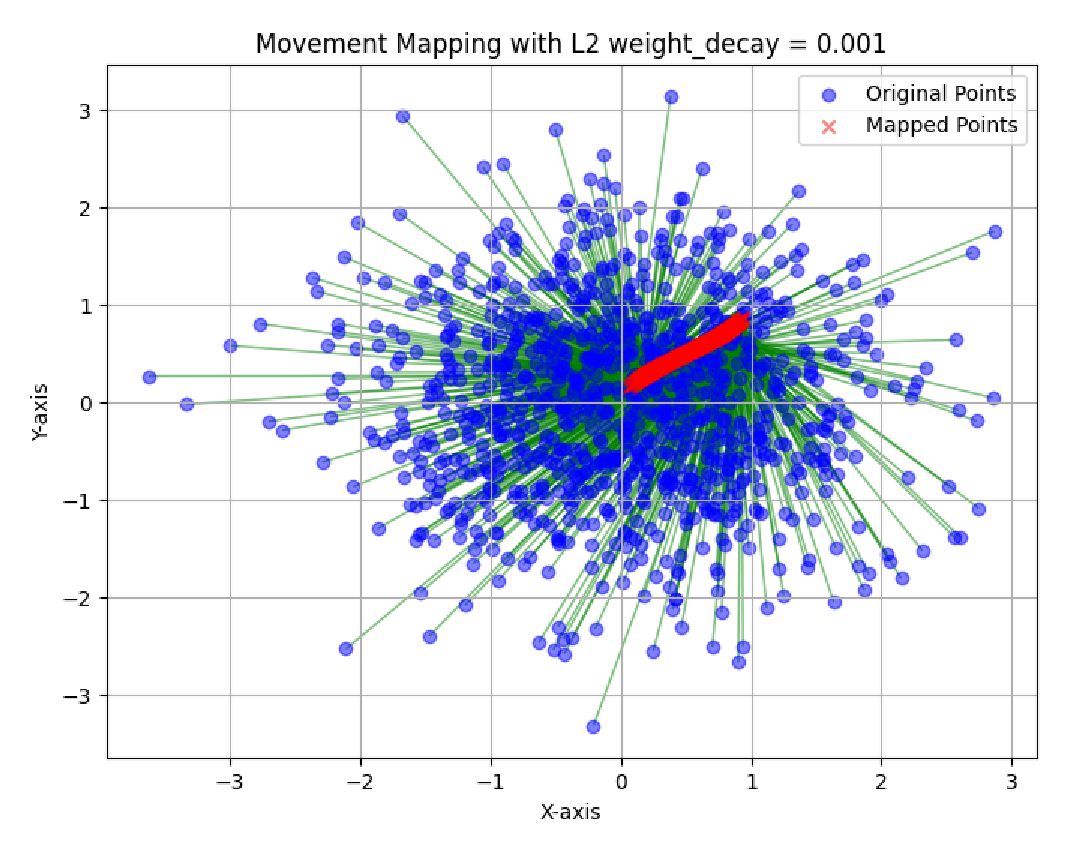
\includegraphics[width=2.5cm]{images/q3_1e-3}}
  %  \vspace{1.5cm}
    \centerline{(c) Points movement with 1e-3}\medskip
  \end{minipage}
  %
  %
  \begin{minipage}[b]{.48\linewidth}
    \centering
    \centerline{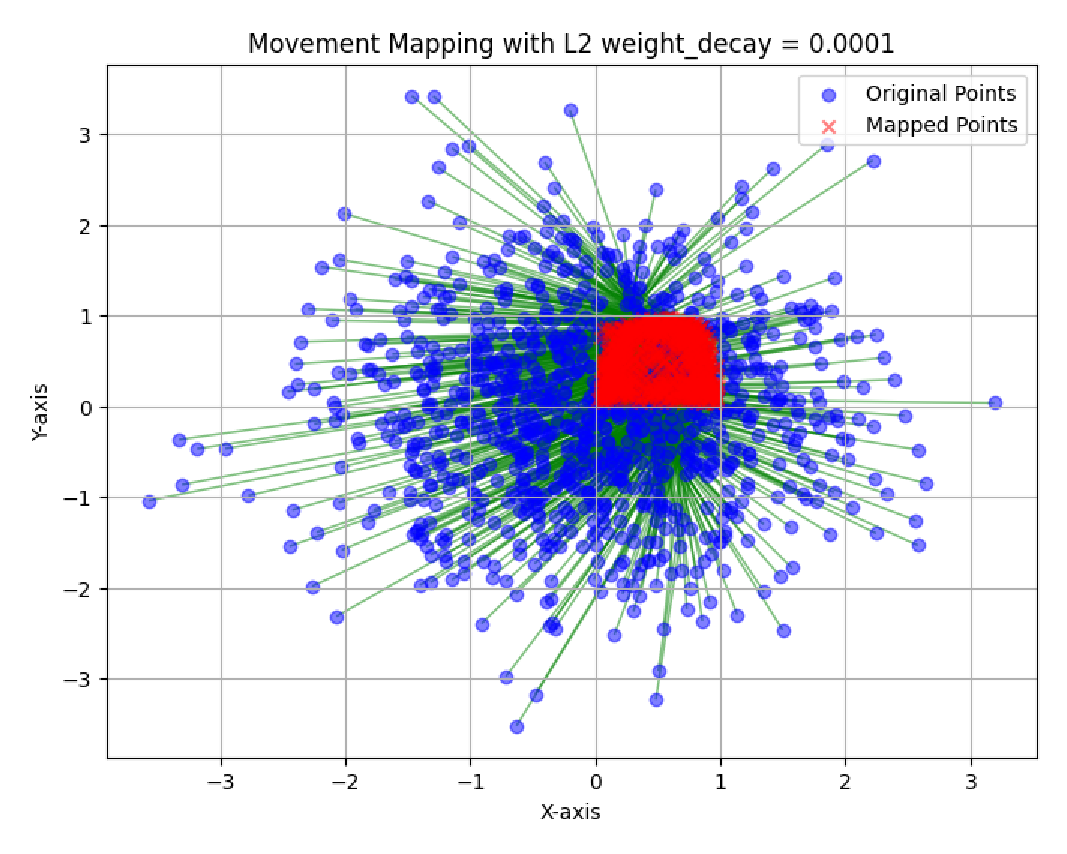
\includegraphics[width=2.5cm]{images/q3_1e-4}}
  %  \vspace{1.5cm}
    \centerline{(d) Points movement with 1e-4}\medskip
  \end{minipage}
  \hfill
  \begin{minipage}[b]{0.48\linewidth}
    \centering
    \centerline{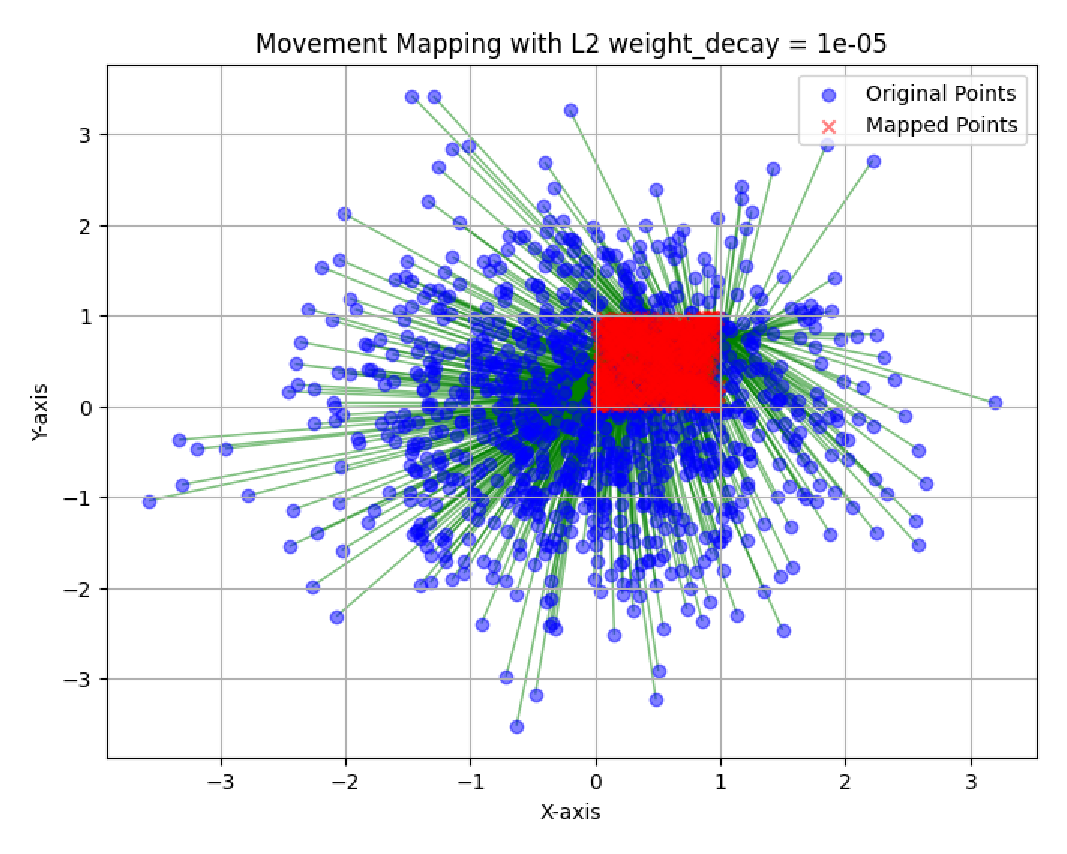
\includegraphics[width=2.5cm]{images/q3_1e-5}}
  %  \vspace{1.5cm}
    \centerline{(e) Points movement with 1e-5}\medskip
  \end{minipage}
  %
  \caption{visulization of dataset}
  \label{fig:q3}
  %
  \end{figure}

\subsection{Using colour plots (various options), discuss what happens to individual
input data points if we concatenate two networks f2 ◦ f1 (mapping
Gaussian to Gaussian) with different L2 regularizations. Discuss the
movement of adjacent points and the effect of the regularization.}
\label{ssec:q4}

In our prior analysis, 
the $f1$ model with $L2$ weight $ < 1\times10^{-4}$ wasn't optimal. 
So, we examined L2 weights of $1\times10^{-4}$, $1\times10^{-5}$, 
$1\times10^{-7}$, and $1\times10^{-8}$. 
Figure $\ref{fig:q4}$ shows the actual Z distribution, 
and Figures $\ref{fig:q4}$ b-e display predictions from $f2$ ◦ $f1$ model. 
Smaller L2 weights in $f1$ yield more restricted prediction ranges, 
whereas larger ones align predictions with the genuine distribution. 
Notably, L2 weight significantly affects the concatenated model's outcomes, 
not just $f1$ alone.

\begin{figure}[htb]
  \begin{minipage}[b]{1.0\linewidth}
    \centering
    \centerline{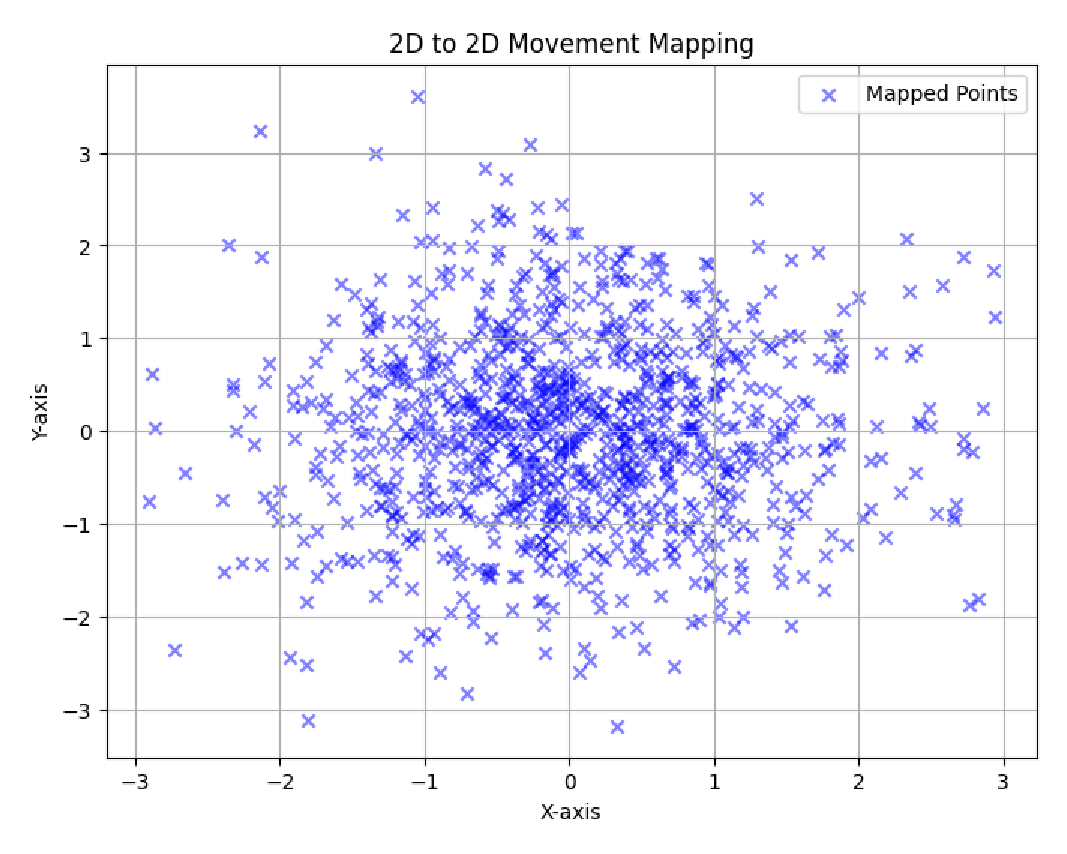
\includegraphics[width=2.5cm]{images/q4_act}}
   %\vspace{2.0cm}
   \centerline{(a) actual distribution of Z }\medskip
  \end{minipage}
  %
  \begin{minipage}[b]{.48\linewidth}
    \centering
    \centerline{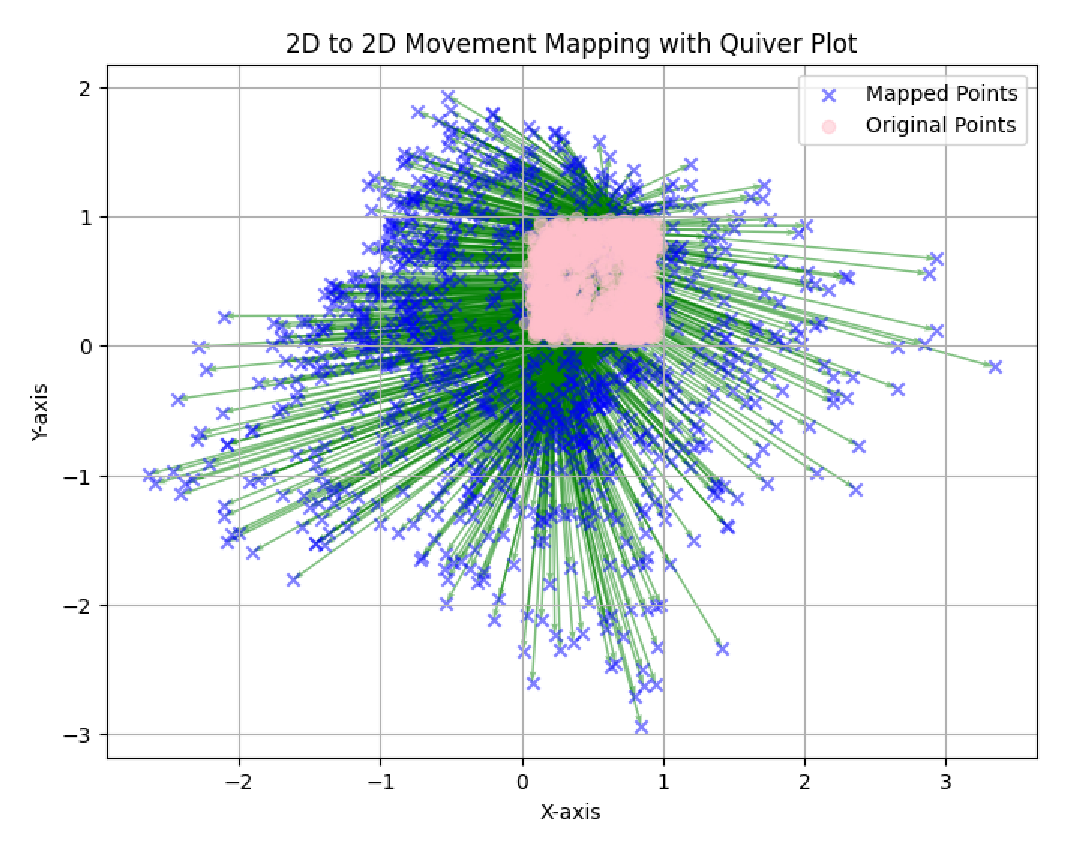
\includegraphics[width=2.5cm]{images/q4_pred_1e-4}}
  %  \vspace{1.5cm}
    \centerline{(a) Points movement with 1e-4}\medskip
  \end{minipage}
  \hfill
  \begin{minipage}[b]{0.48\linewidth}
    \centering
    \centerline{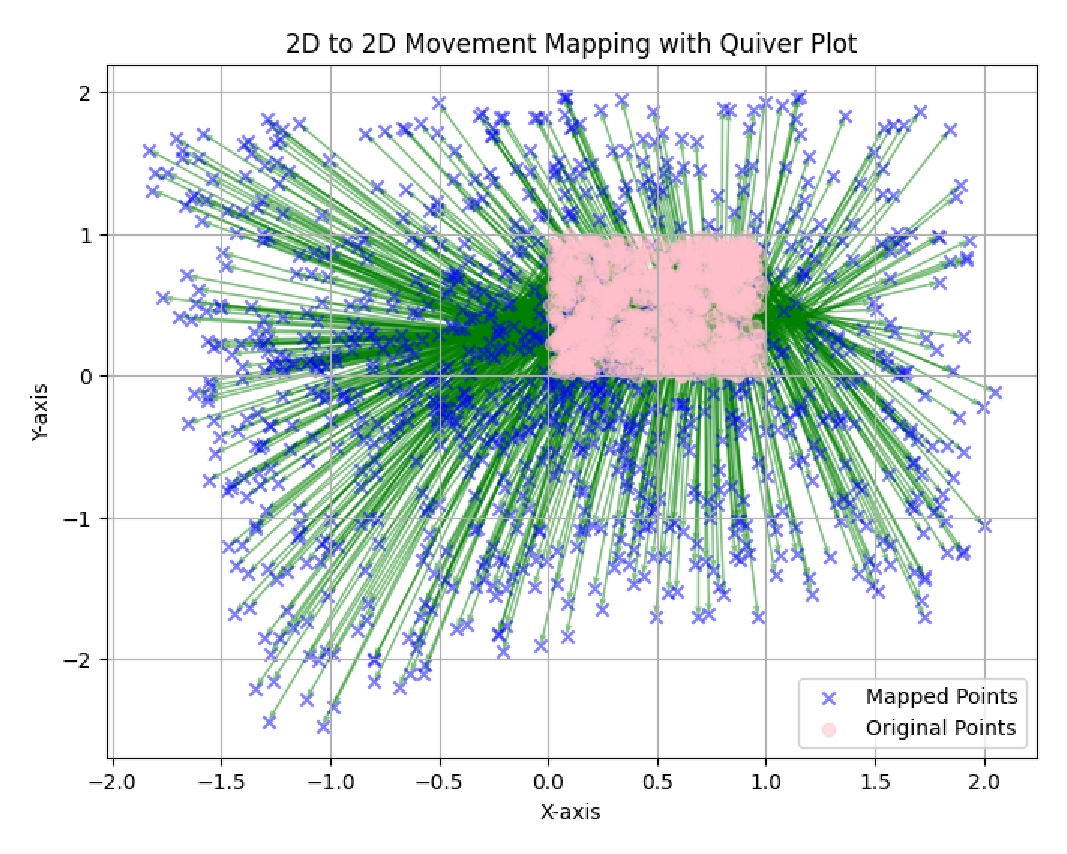
\includegraphics[width=2.5cm]{images/q4_pred_1e-5}}
  %  \vspace{1.5cm}
    \centerline{(c) Points movement with 1e-5}\medskip
  \end{minipage}
  %
  %
  \begin{minipage}[b]{.48\linewidth}
    \centering
    \centerline{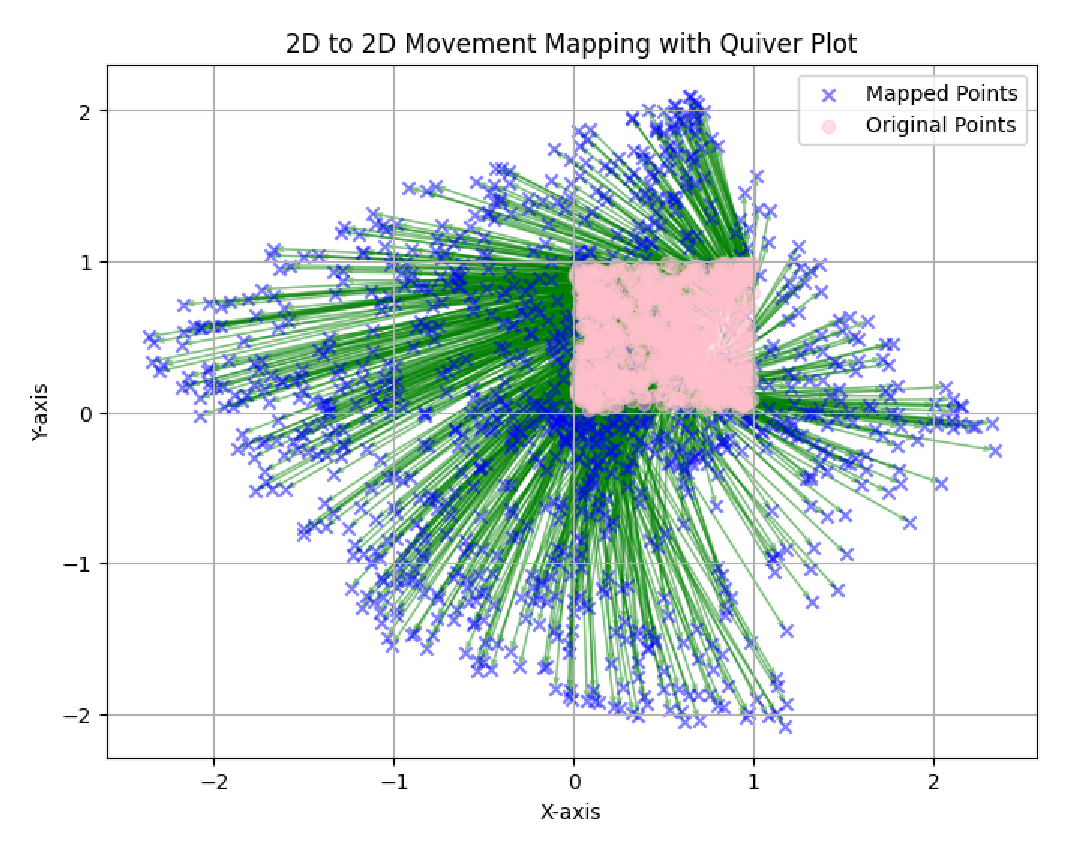
\includegraphics[width=2.5cm]{images/q4_pred_1e-7}}
  %  \vspace{1.5cm}
    \centerline{(d) Points movement with 1e-7}\medskip
  \end{minipage}
  \hfill
  \begin{minipage}[b]{0.48\linewidth}
    \centering
    \centerline{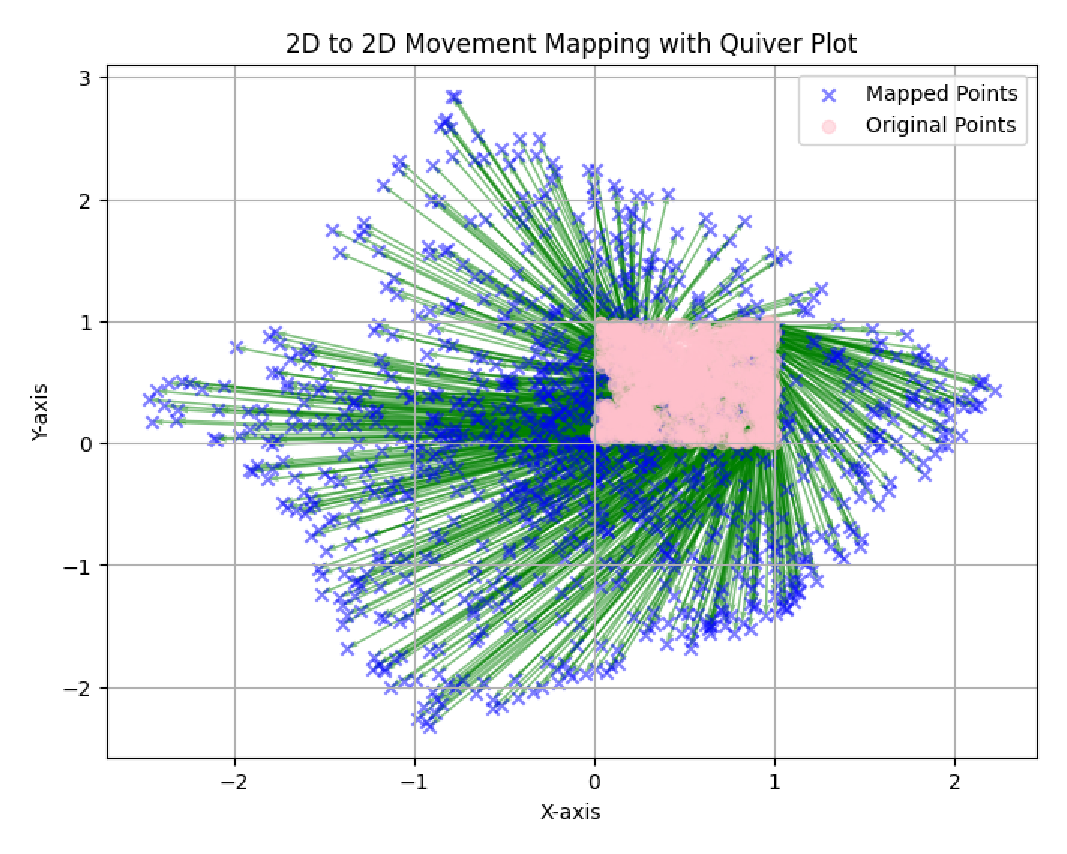
\includegraphics[width=2.5cm]{images/q4_pred_1e-8}}
  %  \vspace{1.5cm}
    \centerline{(e) Points movement with 1e-8}\medskip
  \end{minipage}
  %
  \caption{visulization of dataset}
  \label{fig:q4}
  %
  \end{figure}

\subsection{Train a third network f3 that converts a 1D uniform Y
into a gaussian 2D Z. 
Again use colour plots that show how points are mapped from
the input Y to the output Z}
\label{ssec:q5}

We trained the model $f3$ using a 3-layer NN. 
MMD with a Gaussian Kernel was the loss function. 
We used the Adam optimizer for GD. 
Dropout was added for regularization. 
Figure $\ref{fig:q5}$a (left) shows mapping from input $Y$ to output $Z$ 
and Figure $\ref{fig:q5}$b (right) from input $Y$ to a prior stage. 
Despite similarities, closer inspection reveals differences in 
point mappings, highlighting the diagnostic value of such plots.


\begin{figure}[htb]
  %
  \begin{minipage}[a]{.48\linewidth}
    \centering
    \centerline{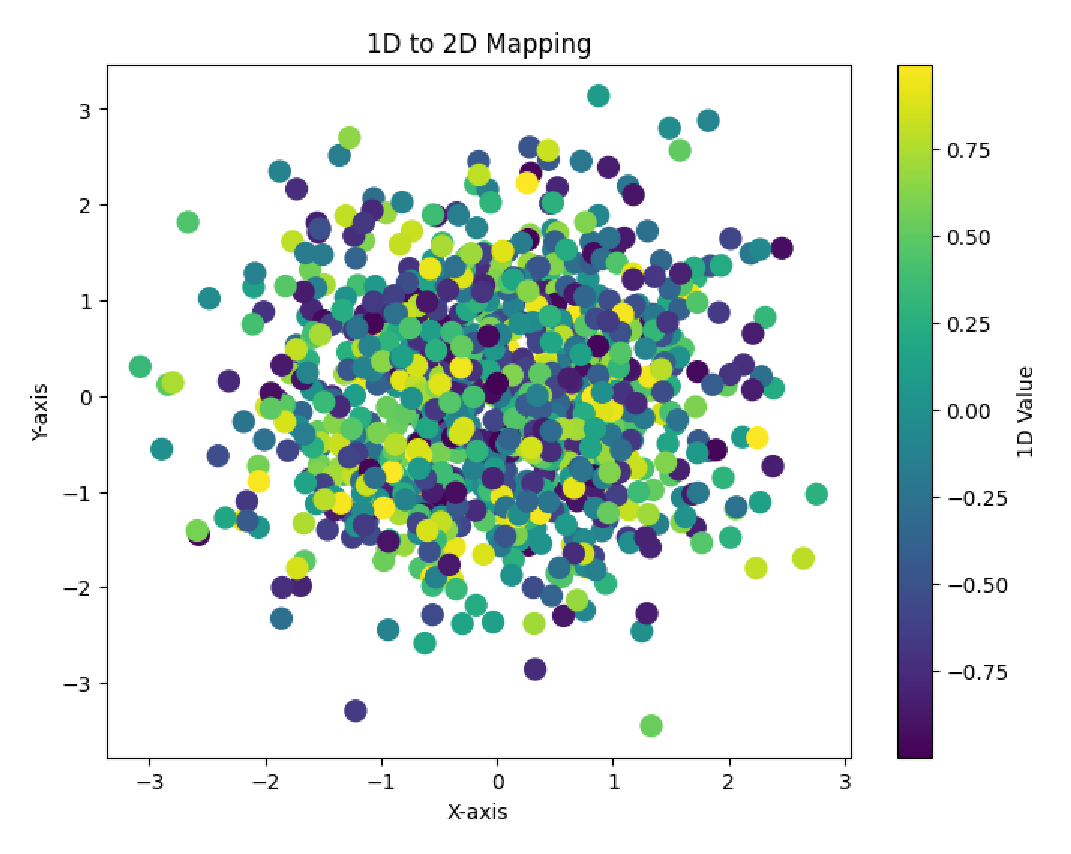
\includegraphics[width=2.5cm]{images/q5_1}}
  %  \vspace{1.5cm}
    \centerline{(a) mapping of output}\medskip
  \end{minipage}
  \hfill
  \begin{minipage}[c]{0.48\linewidth}
    \centering
    \centerline{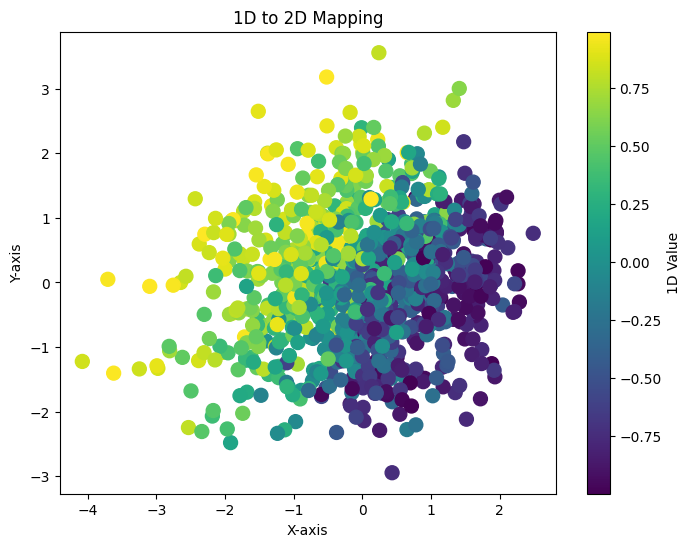
\includegraphics[width=2.5cm]{images/q5_2}}
  %  \vspace{1.5cm}
    \centerline{(b) mapping of prediction}\medskip
  \end{minipage}
  %
  \caption{Points mapped of Model 3}
  \label{fig:q5}
  %
  \end{figure}

\section{CONCLUSION}
\label{sec:conclusion}

From our experimental findings, we determined that color plots are valuable for indicating results in generative models. 
The regularization weight significantly impacts model performance. 
In the concatenated model, the weight of the initial model influences the entire concatenated model's results, even though this weight might not have a pronounced effect on the first model in isolation.

\section{STATEMENT OF ALL TOOLS USED}
\label{sec:statementofalltoolsused}

In this work, we used Pytorch to create, train models. 
The Plotly package helped us visualize in 3D. 
We used scipy.stats to generate the random variables.

Source codes are published in github: 
We run notebook in Colab $\href{https://github.com/felixzhao/AIML425-ASSN-2}{URL}$



% To start a new column (but not a new page) and help balance the last-page
% column length use \vfill\pagebreak.
% -------------------------------------------------------------------------
%\vfill
%\pagebreak

\vfill\pagebreak

% References should be produced using the bibtex program from suitable
% BiBTeX files (here: strings, refs, manuals). The IEEEbib.bst bibliography
% style file from IEEE produces unsorted bibliography list.
% -------------------------------------------------------------------------
\bibliographystyle{IEEEbib}
\bibliography{strings,refs}

\end{document}
